\documentclass[11pt]{article}
\usepackage[hyperref]{acl2023}
\usepackage{times}
\usepackage{latexsym}
\usepackage{microtype}
\usepackage{booktabs}
\usepackage{graphicx}
\usepackage{amsmath}
\usepackage{multirow}
\usepackage[T1]{fontenc}
\usepackage[utf8]{inputenc}

\title{Stylistic Drift as a Model Fingerprint:\\
Measuring Prompt-Invariant LLM Signatures\\
in French Literary Rewrites}

\author{
  Riad Maouchi \\
  \texttt{riad.maouchi@gmail.com}
}

\begin{document}
\maketitle

% ─────────────────────────────────────────────
\begin{abstract}
We study stylistic drift in LLM-rewritten French literary texts using
function-word frequency vectors.
For each original–rewrite pair, we define \emph{shift} as the cosine
distance between their L2-normalised 57-dimensional style vectors, and
compare four commercial models (GPT-4o, Claude Sonnet~4.6,
Mistral Small, Gemini~2.5~Flash) across 80 texts from Zola and Maupassant
and two rewriting prompts.
Three findings emerge.
First, Gemini produces significantly larger stylistic drift than the other
models ($\Delta = 0.23$, $p < 0.001$ after Bonferroni correction);
GPT-4 and Mistral are statistically indistinguishable ($p = 1.0$).
Second, a linear classifier trained on shift vectors reaches only 36.9\%
accuracy (baseline 25\%), confirming that the signal is weak at the
individual-text level.
Third---and most unexpectedly---inter-prompt robustness is partial:
model rankings are preserved across two semantically distinct prompts,
but per-text Pearson correlations are weak ($r \approx 0.28$--$0.32$)
and \emph{null} for Claude ($r = 0.03$, $p = 0.78$), despite Claude
maintaining an identical mean drift under both prompts.
This dissociation suggests that stylistic fingerprints capture
aggregate distributional tendencies of a model rather than
stable per-document properties.
Code and data: \url{https://github.com/riadmaouchi/llm-style-fingerprints}.
\end{abstract}

% ─────────────────────────────────────────────
\section{Introduction}

Large language models rewrite text fluently.
But do they rewrite \emph{neutrally}?
Prior work on authorship attribution has long established that
function words---articles, pronouns, prepositions, conjunctions---carry
stylistic information that is largely unconscious and difficult to suppress
\citep{mosteller1964,burrows1987,juola2015}.
If LLMs systematically alter the distribution of function words when
paraphrasing, they leave a measurable stylistic imprint on the output.

The dominant framing in recent work is \emph{detection}: given a text,
decide whether it was written or assisted by an LLM
\citep{uchendu2023,sadasivan2023,liang2024}.
We adopt a different perspective.
Rather than asking ``is this AI-generated?'', we ask:
\textit{Is the stylistic fingerprint of an LLM robust to the instruction
it receives?}

This question matters for two reasons.
Practically, if the signature is instruction-dependent, detection
methods trained on one prompt will generalise poorly.
Theoretically, it bears on what a ``style'' actually is for an LLM:
a stable latent property of the model, or an emergent pattern
driven by the interaction between model and prompt.

We operationalise stylistic drift as the cosine distance between
the function-word frequency vectors of an original text and its rewrite
(\S\ref{sec:method}), and compare four commercial models
across 80 French literary excerpts and two prompts.
Our main contributions are:

\begin{enumerate}
  \item A reproducible framework for measuring LLM stylistic drift on
    a French literary corpus (40 Zola + 40 Maupassant excerpts, $\sim$120
    words each), with all API outputs archived.
  \item Evidence that model rankings are preserved across prompts but
    per-text correlations are weak, with Claude showing \emph{no}
    significant per-text correlation ($r = 0.03$) despite an identical
    mean drift---a dissociation not previously reported.
  \item A negative result: a logistic classifier on shift vectors
    reaches only 36.9\% accuracy on a 4-class problem (baseline 25\%),
    suggesting that individual-text stylometric fingerprinting of
    LLMs remains unreliable at current corpus sizes.
\end{enumerate}

% ─────────────────────────────────────────────
\section{Related Work}

\paragraph{Authorship attribution and function words.}
The use of function-word frequencies for authorship attribution
dates to \citet{mosteller1964} and was formalised by
\citet{burrows1987}'s Delta method.
\citet{juola2015} demonstrated that four such features sufficed to
identify J.~K.~Rowling behind the pseudonym Robert Galbraith.
\citet{stamatatos2009} provides a comprehensive survey.

\paragraph{LLM-generated text detection.}
\citet{uchendu2023} benchmark multiple detectors across generative models;
\citet{sadasivan2023} prove fundamental detection limits under paraphrase
attacks.
\citet{liang2024} show that detectors exhibit false-positive bias
against non-native speakers---a critical failure mode for applied systems.
Our work differs: we do not build a detector but measure the \emph{degree}
and \emph{structure} of stylistic change.

\paragraph{LLM style and rewriting.}
\citet{guo2023} compare ChatGPT outputs to human experts across domains;
\citet{zhu2023} show that casual paraphrasing can defeat detectors.
Closest to ours is work on style transfer evaluation
\citep{mir2019,tikhonov2019}, which uses function-word features to
assess style preservation.
To our knowledge, no prior work specifically measures the
\emph{per-text correlation} of LLM stylistic shift across prompts,
nor reports the dissociation we observe in Claude.

% ─────────────────────────────────────────────
\section{Method}
\label{sec:method}

\subsection{Corpus}

We use 80 French literary excerpts: 40 from Zola
(\textit{Germinal}, \textit{L'Assommoir}, \textit{Nana},
\textit{La Bête humaine}, \textit{La Débâcle}, and others)
and 40 from Maupassant
(\textit{Boule de suif}, \textit{La Parure}, \textit{Yvette},
\textit{Miss Harriet}, and others).
Each excerpt contains approximately 120 words,
above the 80-word threshold below which we observe signal degradation
(\S\ref{sec:results}).
All texts are in the public domain.

\subsection{Rewriting Prompts}

Each excerpt is rewritten by four commercial LLMs under two prompts:

\begin{itemize}
  \item \textbf{P1} (neutralisation): \textit{``Réécris ce texte dans un
    style neutre et factuel, en conservant le sens.''}
  \item \textbf{P2} (simplification): \textit{``Reformule ce texte en
    simplifiant le vocabulaire, pour le rendre accessible au grand public.''}
\end{itemize}

The four models are GPT-4o, Claude Sonnet~4.6, Mistral Small
(\texttt{mistral-small-latest}), and Gemini~2.5~Flash.
All calls use temperature 0.7 and a maximum of 1\,500 output tokens.
The 640 rewrites (80 texts $\times$ 2 prompts $\times$ 4 models)
are archived in the repository.

\subsection{Style Vectors and Shift}

Following the function-word tradition \citep{burrows1987,stamatatos2009},
we represent each text as a 57-dimensional vector of relative
function-word frequencies (articles, pronouns, prepositions, conjunctions,
and a curated set of discourse markers associated with formal register:
\textit{tandis, pourtant, néanmoins, notamment, afin}).
Vectors are L2-normalised.

The \emph{stylistic shift} of a rewrite $t'$ with respect to its
original $t$ is:
\begin{equation}
  \delta(t, t') = 1 - \frac{v(t) \cdot v(t')}{\|v(t)\|\,\|v(t')\|}
\end{equation}
where $v(\cdot)$ denotes the style vector.
A shift of 0 indicates identical function-word profiles;
a shift of 1 indicates maximal divergence.

We also define a \emph{shift vector} $\mathbf{s} = v(t') - v(t)$,
which captures the \emph{direction} of the stylistic change
in addition to its magnitude.
Shift vectors are used as features for the LDA projection and classifier.

\subsection{Statistical Tests}

Pairwise comparisons use Welch's $t$-test with Bonferroni correction
across all $\binom{4}{2} = 6$ pairs.
Bootstrap confidence intervals (95\%) are computed with $n = 5\,000$
resamples.
Inter-prompt robustness is measured by Pearson $r$ between the
per-text shift series under P1 and P2 for each model.

% ─────────────────────────────────────────────
\section{Results}
\label{sec:results}

\subsection{Stylistic Drift under P1}

Table~\ref{tab:shifts} reports mean shift and bootstrap confidence
intervals for each model under P1.
Gemini produces the largest drift by a substantial margin
($\Delta = 0.230$), while GPT-4 and Mistral are nearly identical
($\Delta = 0.132$ and $0.139$ respectively).

\begin{table}[h]
\centering
\small
\begin{tabular}{lcc}
\toprule
\textbf{Model} & \textbf{Mean shift} & \textbf{95\% CI} \\
\midrule
Gemini 2.5 Flash   & 0.230 & [0.204, 0.256] \\
Claude Sonnet 4.6  & 0.170 & [0.147, 0.195] \\
Mistral Small      & 0.139 & [0.124, 0.157] \\
GPT-4o             & 0.132 & [0.113, 0.152] \\
\bottomrule
\end{tabular}
\caption{Mean cosine shift (P1) and 95\% bootstrap CI ($n = 80$).}
\label{tab:shifts}
\end{table}

Pairwise Bonferroni-corrected tests (Table~\ref{tab:pairwise}) show
that Gemini is significantly different from all other models
($p < 0.01$ in all three comparisons), while GPT-4 and Mistral
are indistinguishable ($p = 1.0$) and Claude occupies an
intermediate, non-significant position.

\begin{table}[h]
\centering
\small
\begin{tabular}{llcc}
\toprule
\textbf{Pair} & & \textbf{$p_{\text{corr}}$} & \textbf{Sig.} \\
\midrule
GPT-4     & vs Gemini  & $<0.001$ & \checkmark \\
Mistral   & vs Gemini  & $<0.001$ & \checkmark \\
Claude    & vs Gemini  & $0.007$  & \checkmark \\
GPT-4     & vs Claude  & $0.103$  & \\
Claude    & vs Mistral & $0.262$  & \\
GPT-4     & vs Mistral & $1.000$  & \\
\bottomrule
\end{tabular}
\caption{Pairwise Welch $t$-tests, Bonferroni-corrected ($k = 6$).}
\label{tab:pairwise}
\end{table}

\subsection{LDA Projection and Classification}

We project shift vectors onto the two leading Linear Discriminant
Analysis (LDA) components.
The LDA projection (Figure~\ref{fig:lda}) reveals that GPT-4 and
Mistral share an almost identical centroid, while Gemini occupies
a clearly separated region.
Claude is intermediate, with substantial overlap with both clusters.

A nearest-centroid classifier (Leave-One-Out) reaches 30.9\% accuracy;
logistic regression on raw shift vectors reaches 36.9\%
(both above the 25\% random baseline).
The primary confusion is between GPT-4 and Mistral,
consistent with the pairwise test result.

\begin{figure}[h]
  \centering
  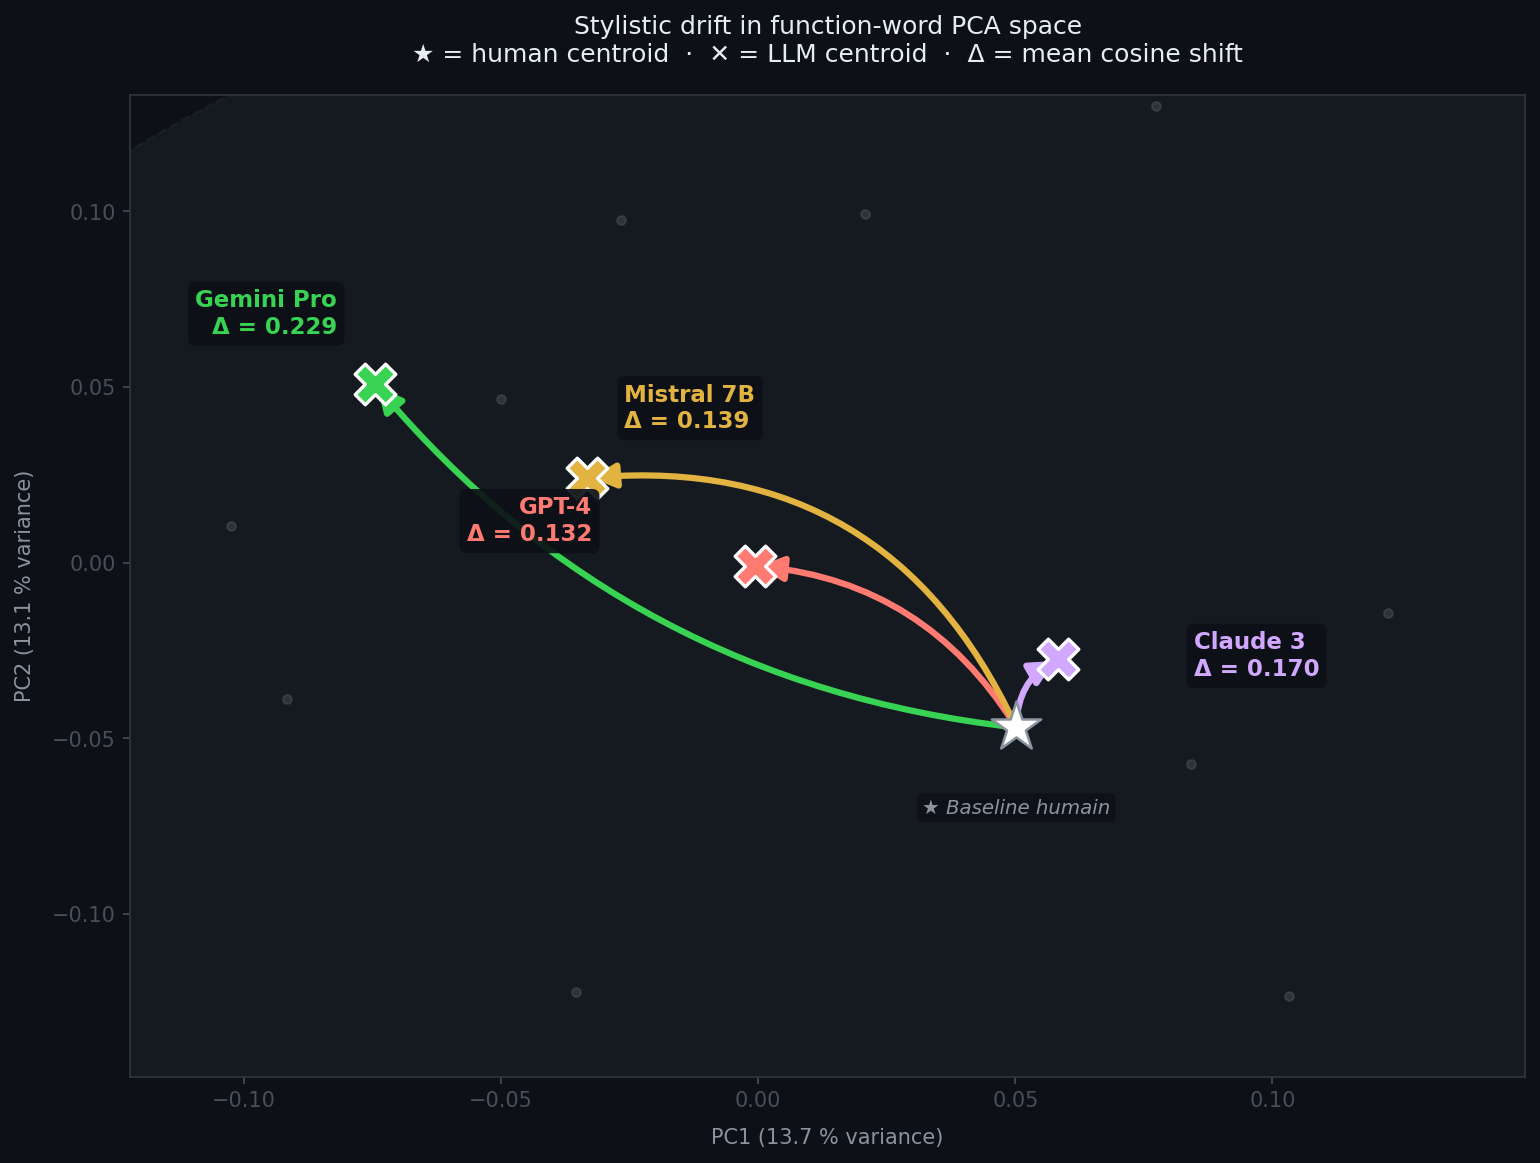
\includegraphics[width=\columnwidth]{../results/drift_trajectories.png}
  \caption{Drift trajectories in LDA shift-vector space.
    Arrows: origin $\to$ model centroid.
    $\Delta$ = mean cosine shift. Ellipses: 1-$\sigma$ dispersion.}
  \label{fig:lda}
\end{figure}

\subsection{Inter-Prompt Robustness}
\label{sec:robustness}

Table~\ref{tab:robustness} reports, for each model, the Pearson
correlation between per-text shift under P1 and P2,
together with the mean shift under each prompt.

\begin{table}[h]
\centering
\small
\begin{tabular}{lcccc}
\toprule
\textbf{Model} & \textbf{$r$} & \textbf{$p$} &
  \textbf{$\bar\delta_{P1}$} & \textbf{$\bar\delta_{P2}$} \\
\midrule
Gemini  & 0.32 & 0.004 & 0.229 & 0.167 \\
Mistral & 0.28 & 0.010 & 0.139 & 0.130 \\
GPT-4   & 0.28 & 0.011 & 0.132 & 0.096 \\
Claude  & 0.03 & 0.778 & 0.170 & 0.176 \\
\bottomrule
\end{tabular}
\caption{Inter-prompt robustness: Pearson $r$ between per-text shifts
  under P1 and P2 ($n = 80$).}
\label{tab:robustness}
\end{table}

Three observations stand out.
First, for GPT-4, Mistral, and Gemini, the correlations are
statistically significant but weak ($r \approx 0.28$--$0.32$):
knowing that a given text was strongly shifted under P1 gives only
modest predictive power for its shift under P2.
Second, P2 consistently produces lower mean shift than P1
for these three models (simplification is less stylistically disruptive
than neutralisation).
Third---the key finding---Claude shows \emph{no} significant
per-text correlation ($r = 0.03$, $p = 0.78$) despite an almost
identical mean shift under both prompts (0.170 vs.\ 0.176).
The texts that Claude displaces most under P1 are essentially
uncorrelated with those it displaces most under P2.

% ─────────────────────────────────────────────
\section{Discussion}

\paragraph{What the Claude dissociation implies.}
The dissociation between mean drift and per-text correlation in Claude
is the most theoretically interesting result.
It rules out the simplest explanation---that the model has a fixed
``aggressiveness'' applied uniformly across texts---and suggests instead
that Claude's stylistic choices are more sensitive to the interaction
between the prompt and the specific text.
Under P1 (neutralise), some texts trigger strong formal register shifts;
under P2 (simplify), a different set of texts is affected.
This is consistent with Claude being more instruction-following
at the sentence level, while Gemini imposes a more
uniform stylistic template regardless of content.

\paragraph{Aggregate ranking vs.\ individual prediction.}
All four models preserve the same relative ranking under P1 and P2
(Gemini $>$ Claude $>$ Mistral $\approx$ GPT-4).
This ranking robustness is meaningful for comparative model evaluation:
the choice of rewriting prompt does not change which model shifts style
the most.
However, it does not license individual-level inference:
a single text rewritten by Claude under P1 is not predictably
more or less shifted than the same text under P2.

\paragraph{Limitations.}
$n = 80$ excerpts from two 19th-century French authors limits
generalisability.
The function-word list includes markers selected partly for
their known association with LLM formal register
(\textit{tandis, néanmoins, notamment}),
introducing a mild bias toward models that use formal connectives.
Finally, all models were queried at a fixed snapshot in time;
model updates may alter these signatures.

% ─────────────────────────────────────────────
\section{Conclusion}

We measured stylistic drift in 640 LLM rewrites of French literary texts
using cosine distance in function-word space.
Gemini produces the largest drift and is the only model
clearly distinguishable from all others.
GPT-4 and Mistral are statistically indistinguishable.
Inter-prompt robustness is partial: model rankings are stable,
but per-text shift correlations are weak, and null for Claude---a
dissociation that suggests stylistic fingerprints reflect
distributional tendencies of models rather than
stable per-document properties.
Individual-text LLM identification via stylometry remains unreliable
at current corpus sizes (36.9\% accuracy, 4 classes).

% ─────────────────────────────────────────────
\section*{Acknowledgements}
All API outputs used in this study are archived at
\url{https://github.com/riadmaouchi/llm-style-fingerprints}.
No human subjects were involved.

% ─────────────────────────────────────────────
\bibliography{refs}

\end{document}
